\section{High Level Considerations}

Before diving into the details of consensus mechanisms, let's take a look at the advantages and limitations of using blockchain:

\begin{table}[h]
\begin{tabularx}{\linewidth}{>{\parskip1ex}X@{\kern4\tabcolsep}>{\parskip1ex}X}
\toprule
\hfil\bfseries \color{Orange}{Pros}
&
\hfil\bfseries \color{Orange}{Cons}
\\\cmidrule(r{3\tabcolsep}){1-1}\cmidrule(l{-\tabcolsep}){2-2}

%% PROS
Among the main benefits, \textbf{\color{Blue}{decentralization}} emerges as one of the key pillars, enabling a distributed network in which no central authority has absolute control. This not only increases the security and reliability of the network, but also promotes \textbf{\color{Blue}{transparency and trust}} among participants, making every transaction traceable and verifiable by anyone. In addition, the \textbf{\color{Blue}{immutability}} of data recorded on the blockchain, coupled with its \textbf{\color{Blue}{high availability}}, ensures that information is protected from manipulation and \textbf{\color{Blue}{always accessible}} when needed. These benefits, along with process simplification, efficiency in regulations and \textbf{\color{Blue}{cost savings}}, turn blockchain into a \textbf{\color{Blue}{reliable and programmable platform}} for a wide range of applications. Specifically, cost savings result from the elimination of intermediaries in transactions, enabling a direct transfer of value between the parties involved.
&

%% CONS
However, despite its advantages, blockchain technology also has some significant limitations that hinder its wider adoption. The appearance of the \textbf{\color{Blue}{new technology}}, for example, poses challenges in terms of familiarization and implementation for many organizations. In addition, the \textbf{\color{Blue}{scalability}} of blockchain, especially in public networks, may be limited with respect to the needs of high-frequency transactions. The issue of data \textbf{\color{Blue}{privacy and confidentiality}} remains an area of concern, as information recorded on the blockchain is permanent and accessible to all participants. \textbf{\color{Blue}{Limited adoption}}, \textbf{\color{Blue}{interoperability}} between different blockchain platforms, and complex \textbf{\color{Blue}{regulatory issues}} represent additional challenges that must be overcome to maximize the potential of blockchain technology.
\\\bottomrule
\end{tabularx}
\caption{Benefits and Limitations of Blockchain Technology.}
\end{table}

\section{DLT Categories}
\textbf{Distributed Ledger Technologies} (DLTs) can be categorized in different ways based on their use and structure. One of the main categories is Blockchain, which is a specific type of DLT used for shared and immutable ledgers.

Blockchain can be further divided into three main types: public, private and consortium. \textbf{\textcolor{Orange}{Public blockchains}} are open to anyone who wants to participate and are decentralized. \textbf{\textcolor{Orange}{Private blockchains}} are controlled by a centralized organization or entity and are accessible only to authorized users. \textbf{\textcolor{Orange}{Consortial blockchains}} are managed by a group of organizations working together to manage the network.

In addition to blockchains, there are other types of DLTs such as Sidechains and Distributed Ledgers. \textbf{\textcolor{Orange}{Sidechains}} are blockchains linked to a main blockchain and can be used for specific purposes or to enhance the functionality (scalability) of the main blockchain. \textbf{\textcolor{Orange}{Distributed Ledgers}}, on the other hand, are shared ledgers that can be customized for specific purposes and are not necessarily blockchain-based.

\begin{figure}[h]
\centering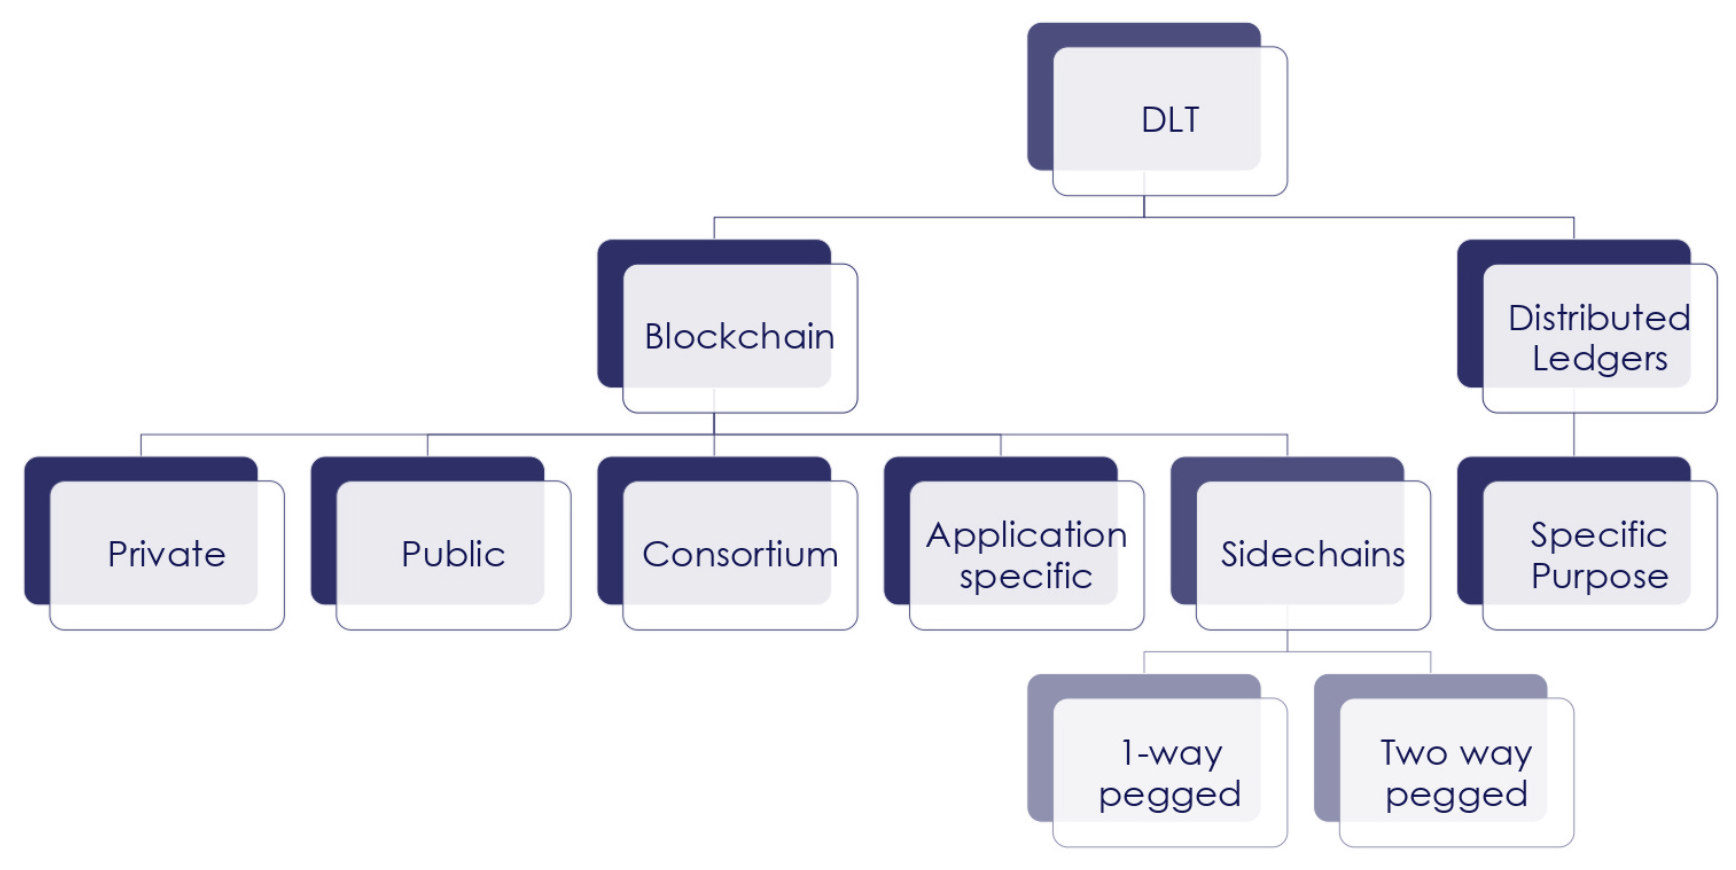
\includegraphics[scale=0.3]{images/chapter3 - DLT.png}
\caption{Distributed Ledger Technologies Categories.}
\end{figure}

\section{Byzantine Generals Problems}
The Byzantine Generals problem (PBFT) is a fundamental concept in the context of distributed consensus mechanisms. Imagine a situation in which several commanders of an army must coordinate to attack or retreat, but some of them may be traitors or communications between them may be compromised. In this scenario, it is essential that the generals reach a consensus on the strategy to be adopted despite the uncertainty and the presence of potential mistakes or sabotage.

PBFT solves this problem by establishing a set of requirements to ensure reliable consensus among participants (Of course, we are no longer talking about battles, but about blockchain!). These requirements include:
\begin{itemize}
    \item \textbf{Agreement}: All nodes must agree on a single value proposition or decision.
    \item \textbf{Integrity}: Information and transactions must be authentic and unchanged during the consensus process.
    \item \textbf{Validity}: Only valid and legitimate transactions must be accepted and confirmed.
    \item \textbf{Fault Tolerance}: The system must be able to function properly even if some nodes fail or misbehave.
    \item \textbf{Termination}: The consensus process must eventually reach a conclusion and produce a final outcome.
\end{itemize}
Using PBFT, participants can collaborate safely and reliably even in the presence of faulty or malicious nodes. This consensus mechanism is critical to ensuring the consistency and reliability of transactions within distributed networks, such as those based on blockchain technology.

\vspace{2cm}
\section{Security Mechanisms}
In the blockchain, the application of security mechanisms is critical to ensure the security and integrity of transactions. These functions are used in different contexts, below we make a list and it is likely that you already know how some of them work.

\begin{remark}
\textbf{Cryptographic Hash Functions}:
Hash functions are fundamental in the blockchain and are used to confirm and validate new blocks of transactions, to create unique addresses for accounts on the blockchain, to verify the authenticity of messages sent over the network and in Merkle trees.
\end{remark}

\begin{remark2}
\textbf{Asymmetric cryptography}:
A cryptographic technique involving two keys: public and private. 
In the encryption process, the sender encrypts the message with the recipient's public key and, in the case of digital signatures, signs the message with his own private key, while the recipient verifies the signature using the sender's public key.
\end{remark2}

\begin{remark}
\textbf{Merkle trees}:
A data structure that ensures the integrity of transactions in the blockchain.
Transactions are organized in a binary tree, and hashes are used to ensure the integrity of the structure.
They allow for quick verification of whether a transaction is included in a blockchain without having to examine all transactions.
\end{remark}


\section{Type of Consensus Mechanisms}
When it comes to exploring the vast world of consensus mechanisms within blockchains, we are faced with a myriad of options. However, we will focus mainly on three of them: the Proof of Work, the Proof of Stake and the Delegated Proof of Stake. 

\faBitcoin \; \textbf{Proof of Work} (PoW):

In PoW, participants, called "miners," compete to solve complex cryptographic puzzles.
The first miner to solve the puzzle gains the right to create and confirm a new block of transactions on the blockchain.
This process requires an enormous amount of computing power, making the system secure but also energy intensive.

\faEthereum \; \textbf{Proof of Stake} (PoS):

In PoS, the right to create and validate a new block depends on the amount of cryptocurrency owned and "played" by participants, called "validators."
The more cryptocurrency that is "played," the greater the probability of being chosen to validate a block and receive rewards.
Because it does not require as intensive computing power as PoW, PoS is more energy efficient.

\faUsers \; \textbf{Delegated Proof of Stake} (DPoS):

In DPoS, participants elect "delegates" responsible for creating and confirming blocks.
These delegates are voted on by other participants based on trust and reputation.
DPoS is designed to scale more efficiently than PoW and PoS, allowing for faster confirmation of transactions.

